\chapter{Технологическая часть}


\section{Средства реализации}
В качестве языка программирования для реализации алгоритмов выбран язык \textit{Rust}~\cite{rustbook}, так как он удовлетворяет всем требования.

Для реализации графического интерфейса использована библиотека \textit{egui}~\cite{egui}.

В качестве среды разработки была выбрана IDE \textit{RustRover}~\cite{rustrover}.


\section{Формат входных и выходных данных}


\section{Реализация алгоритмов}
В данном разделе приведены листинги кода, реализующего основные алгоритмы.

\subsection{Реализация алгортмов растеризации TODO: название}.

На листингах~\ref{lst:z-buf-1},~\ref{lst:z-buf-2} приведена реализация алгоритма отрисовки объекта с использованием \textit{z}-буфера и модифицированной закраски Гуро.

\lstinputlisting[
    caption=Реализация алгоритма отрисовки объекта с использованием \textit{z}-буфера и модифицированной закраски Гуро (часть 1),
    label=lst:z-buf-1,
    firstline=142,
    lastline=181
]{render/z_buffer.rs}

\lstinputlisting[
    caption=Реализация алгоритма отрисовки объекта с использованием \textit{z}-буфера и модифицированной закраски Гуро (часть 2),
    label=lst:z-buf-2,
    firstline=86,
    lastline=140
]{render/z_buffer.rs}

\subsection{Реализация алгоритмов морфинга}

На листинге~\ref{lst:morph-create} представлена реализация алгоритма построения объекта морфинга из исходной и целевой сеток.
\lstinputlisting[
    caption=Реализация алгоритма построения мофринга из исходной и целевой сеток,
    label=lst:morph-create,
    firstline=31,
    lastline=113
]{objects/morph.rs}

На листингах~\ref{lst:mesh-parametrization}--\ref{lst:supermesh-2} представлены реализации алгоритмов основных этапов построения морфинга.

\lstinputlisting[
    caption=Реализация алгоритма сферической параметризации сетки,
    label=lst:mesh-parametrization,
    firstline=180,
    lastline=201
]{utils/morphing.rs}

\lstinputlisting[
    caption=Реализация алгоритма релаксации сетки на единичной сфере,
    label=lst:mesh-relaxation,
    firstline=74,
    lastline=128
]{utils/morphing.rs}

\lstinputlisting[
    caption=Реализация алгоритма релаксации сетки на единичной сфере,
    label=lst:mesh-relaxation,
    firstline=74,
    lastline=128
]{utils/morphing.rs}

\lstinputlisting[
    caption=Реализация алгоритма построения суперсетки (часть 1),
    label=lst:supermesh-1,
    firstline=609,
    lastline=621
]{utils/morphing.rs}

\lstinputlisting[
    caption=Реализация алгоритма построения суперсетки (часть 2),
    label=lst:supermesh-2,
    firstline=375,
    lastline=485
]{utils/morphing.rs}


\section{Интерфейс программы}

На рисунках~\ref{fig:gui-1},~\ref{fig:gui-2} представлен пример работы программы.

\begin{figure}[H]
    \label{fig:gui-1}
    \centering
    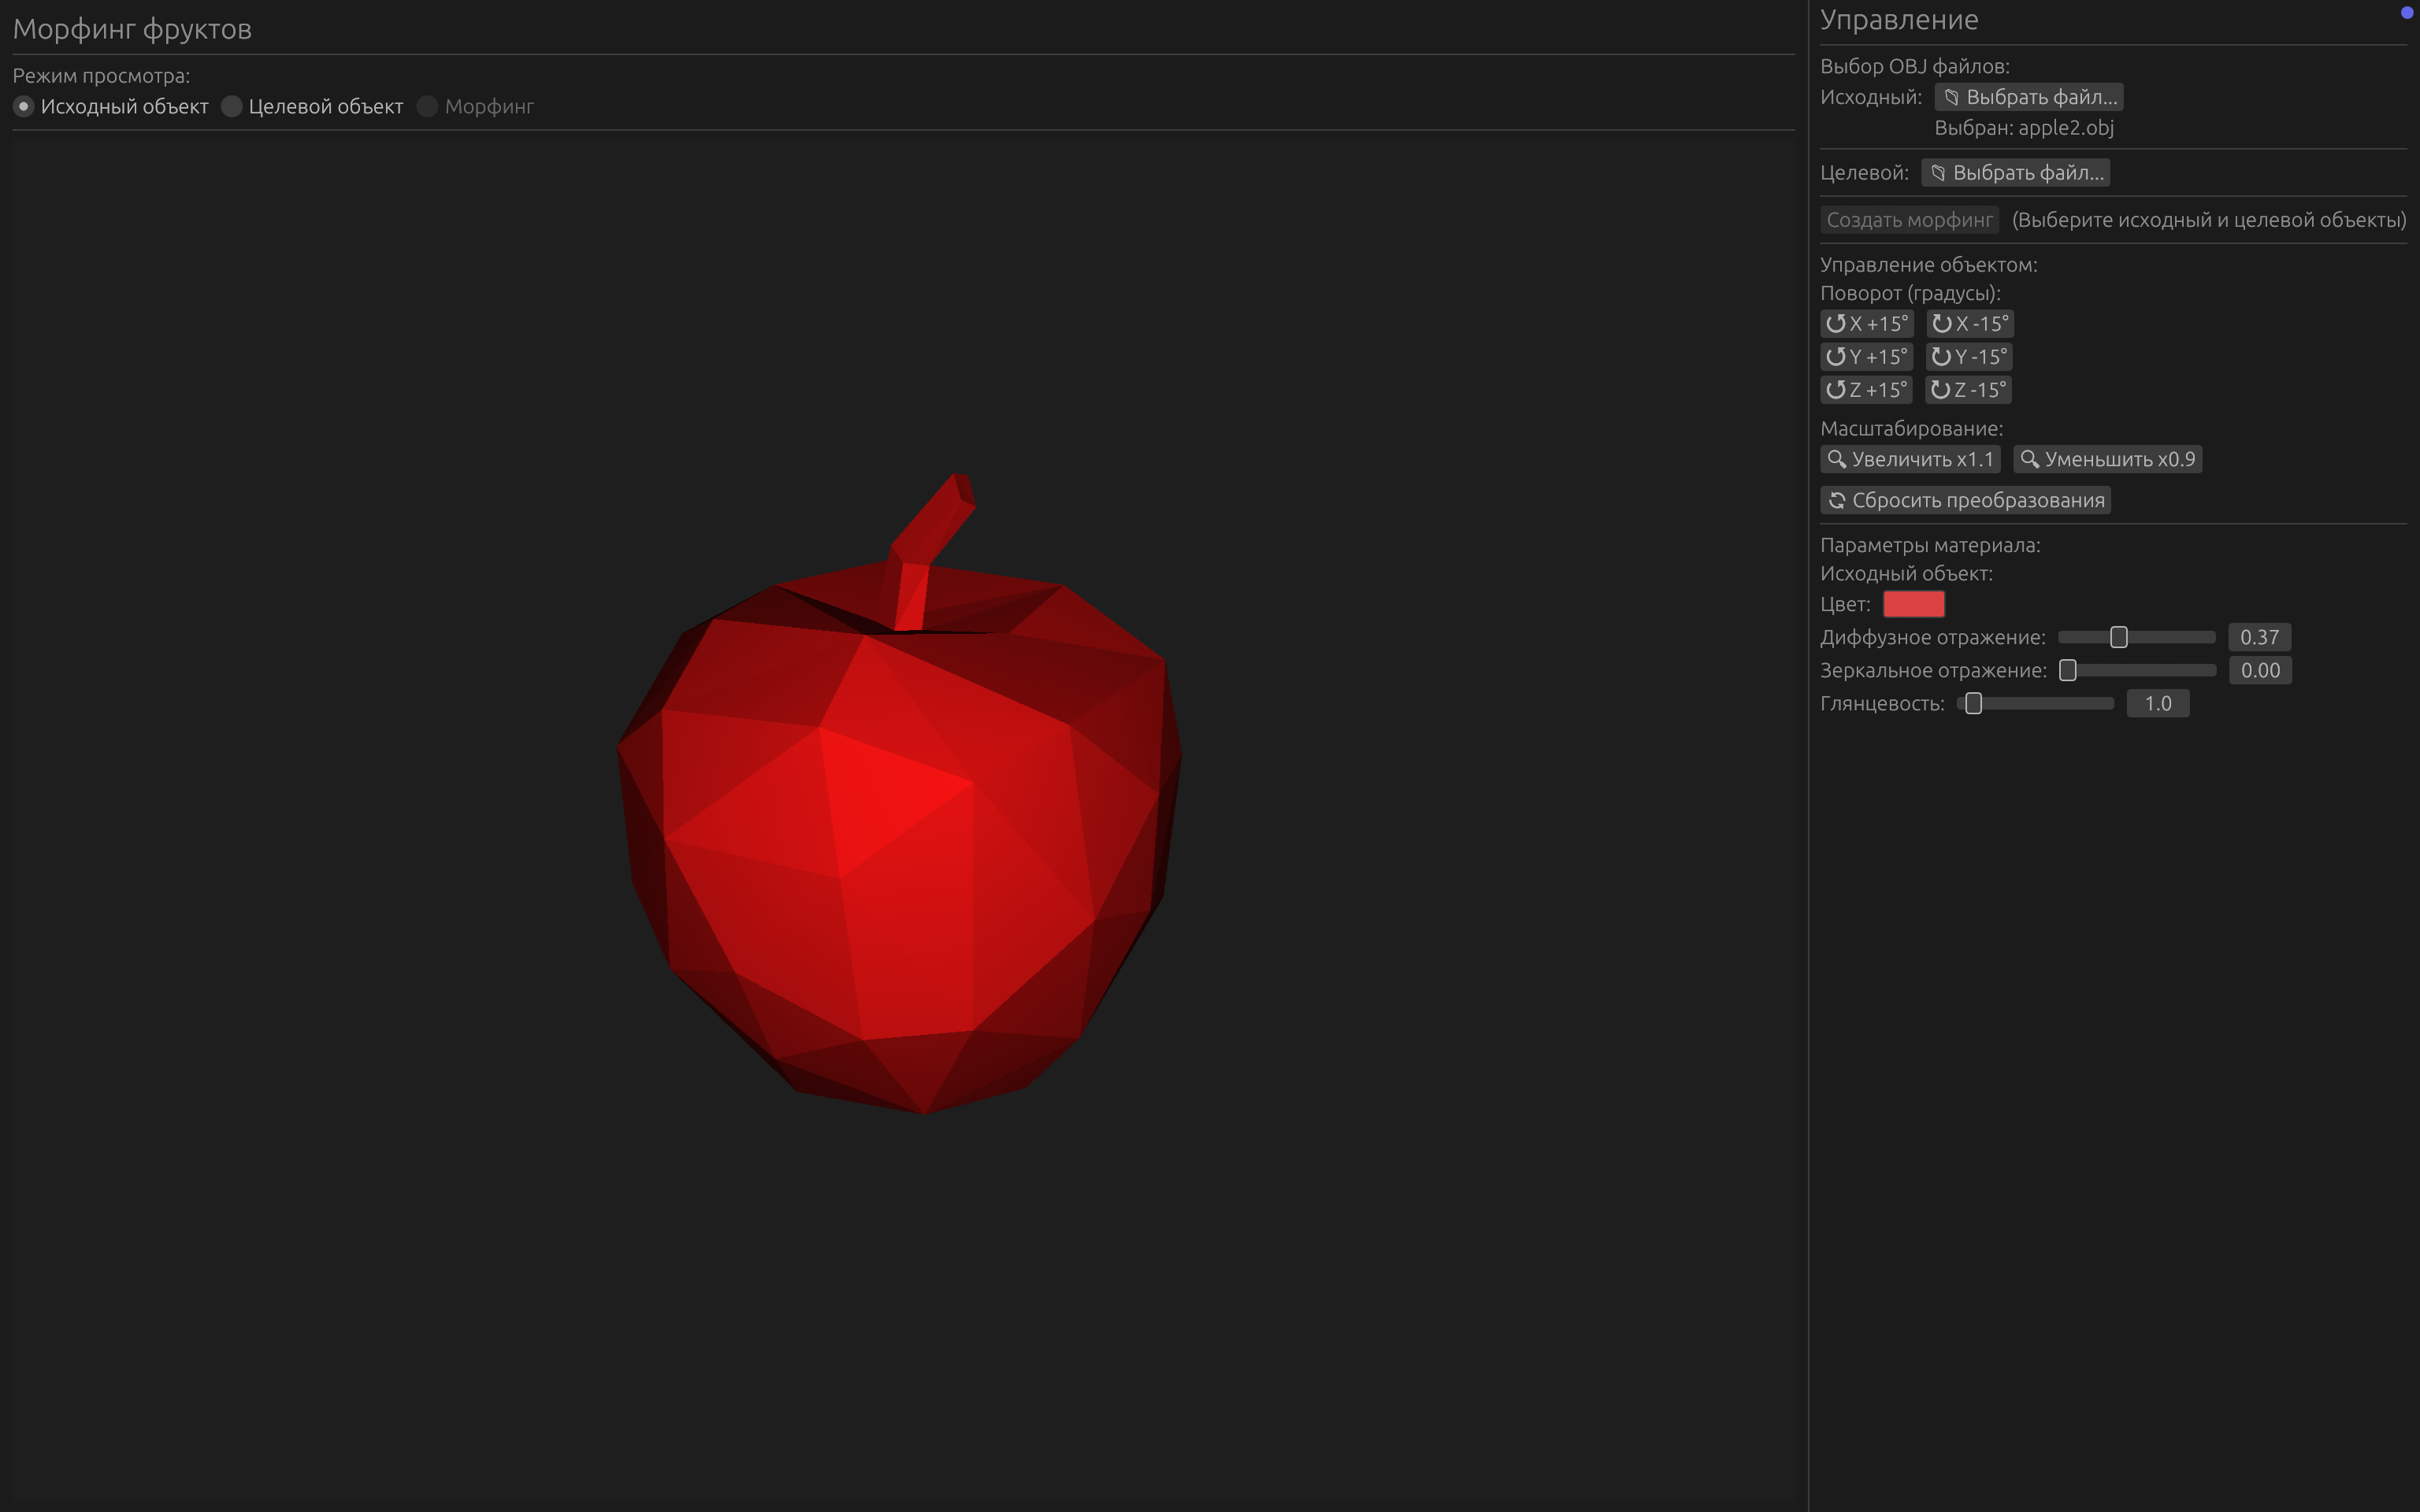
\includegraphics[width=0.8\textwidth]{gui-1}
    \caption{Пример графического интерфейса программы --- управление исходным объеком}
\end{figure}

\begin{figure}[H]
    \label{fig:gui-2}
    \centering
    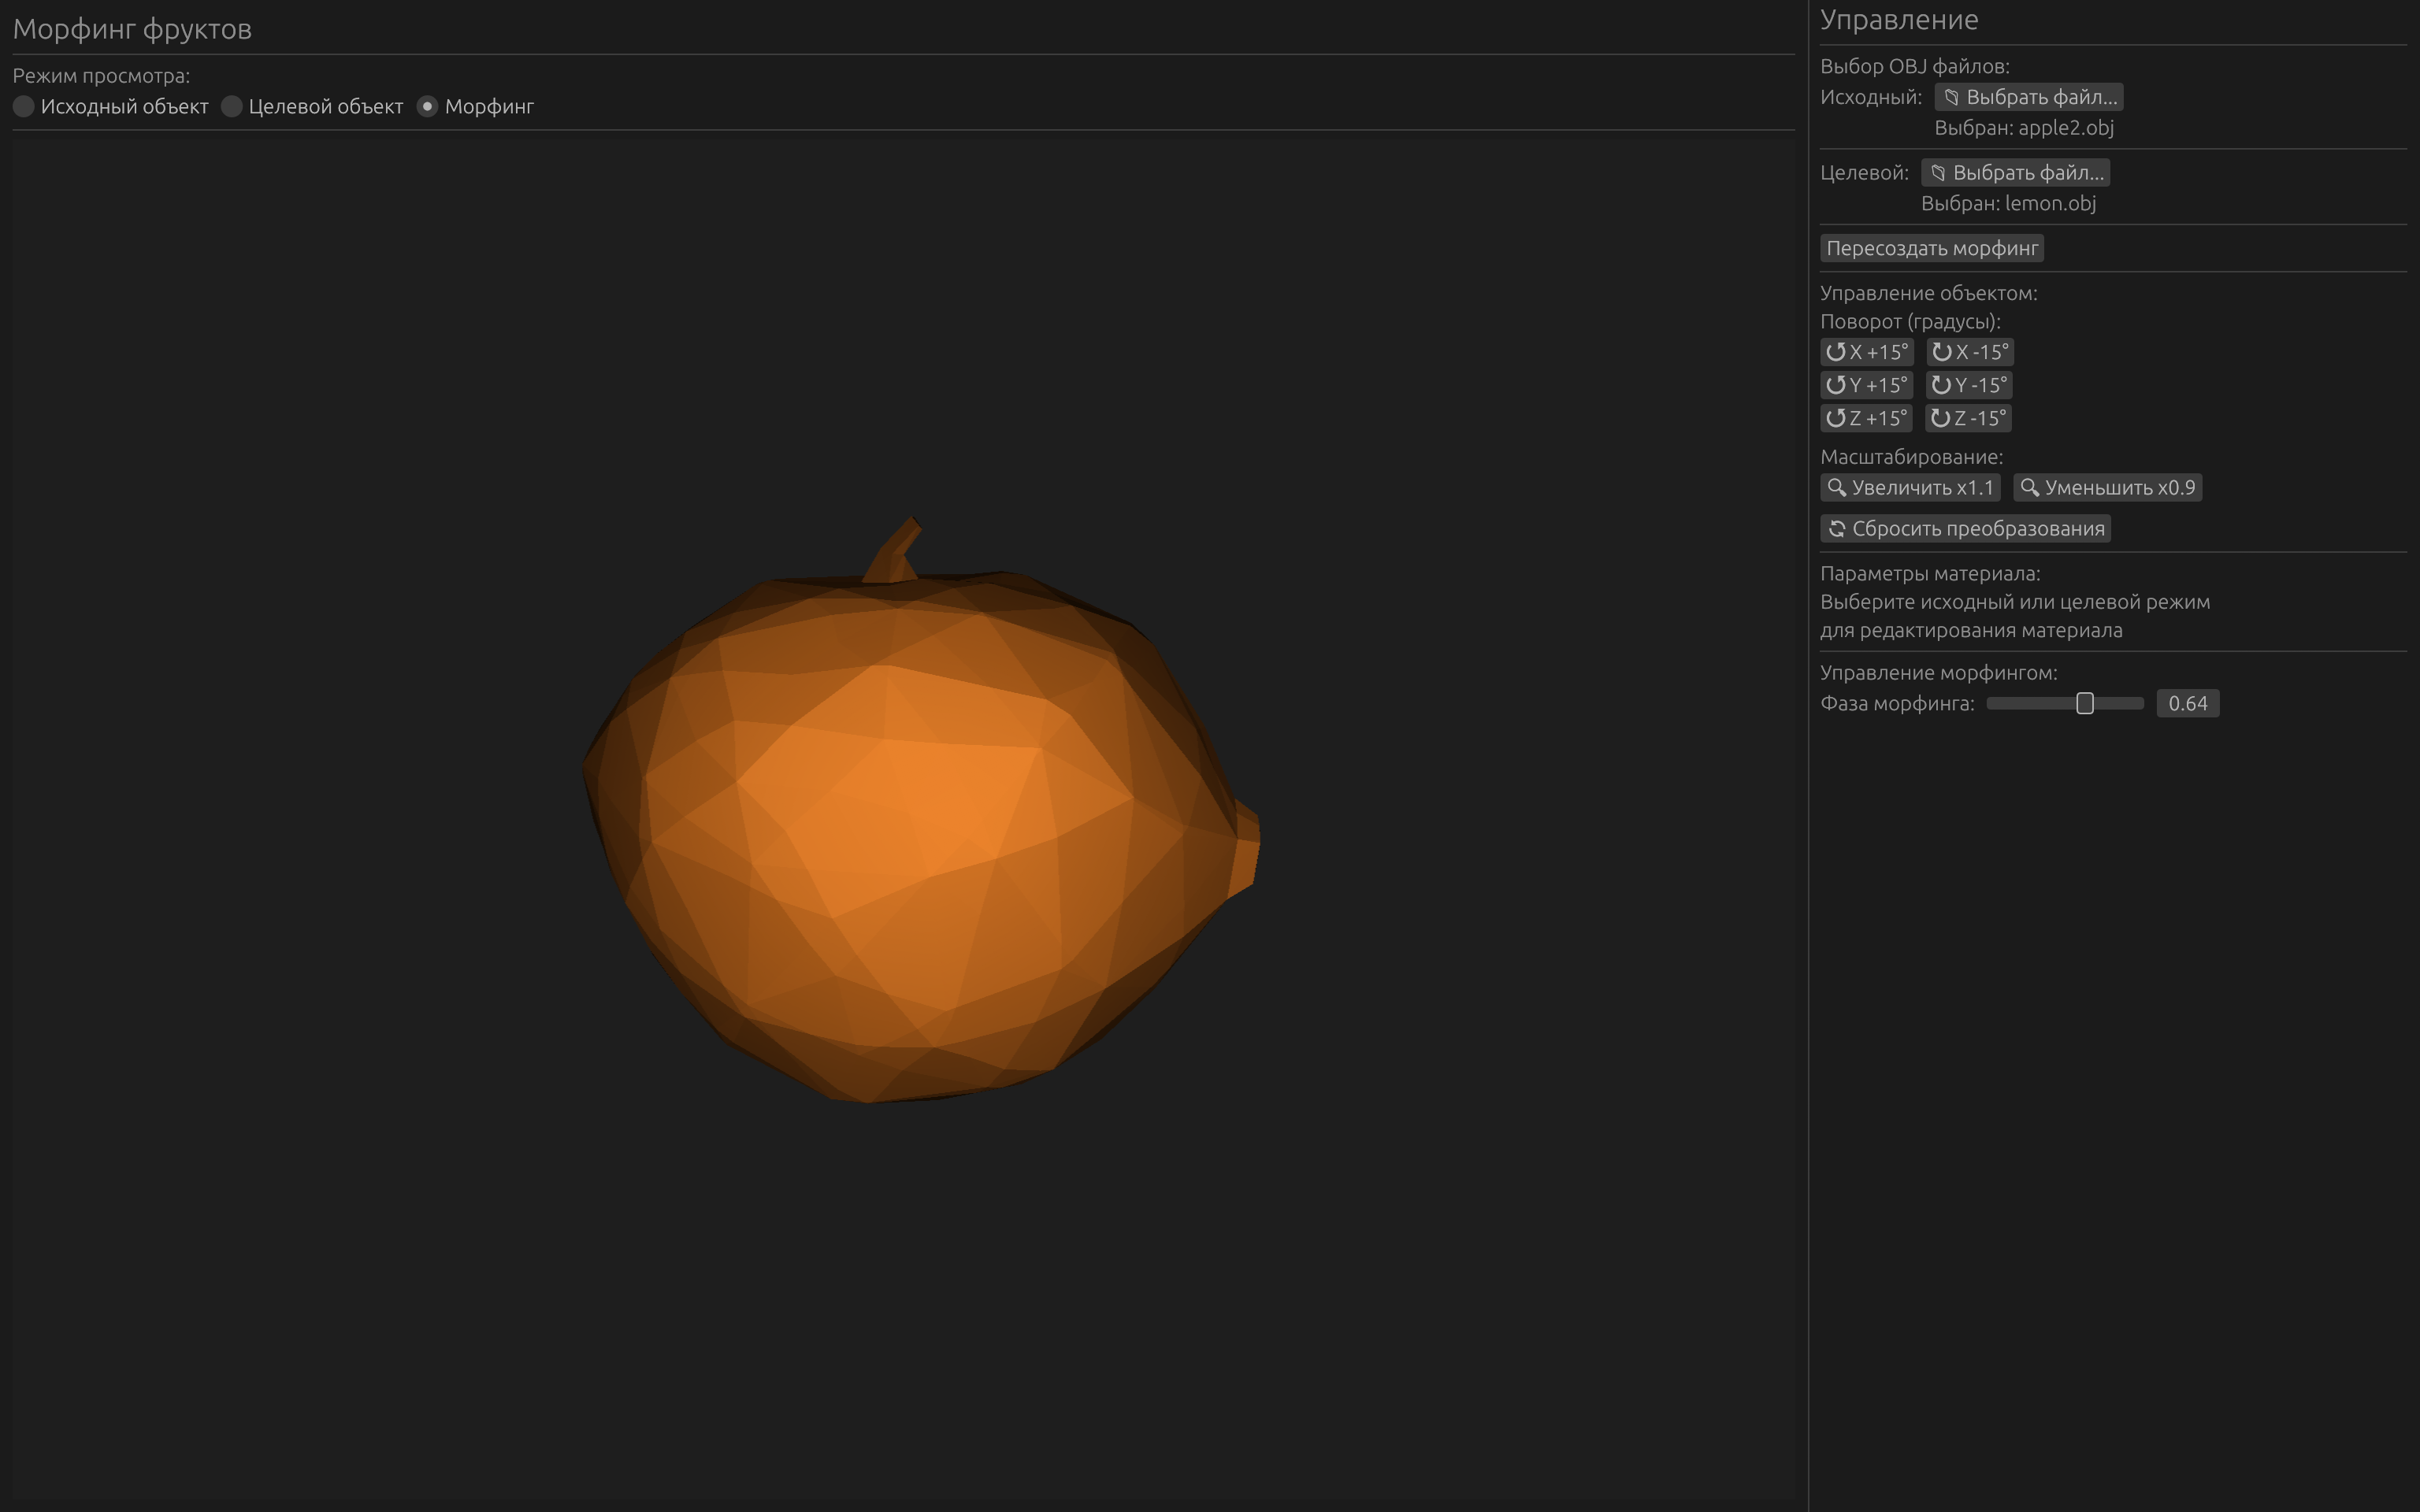
\includegraphics[width=0.8\textwidth]{gui-2}
    \caption{Пример графического интерфейса программы --- управления морфингом}
\end{figure}

Для загрузки объектов используются кнопки <<Загрузить исходный объект>> и <<Загрузить целевой объект>>.

После того как объекты загружены, становятся доступна кнопка <<Создать морфинг>>, по нажатию на которую выполняется построение объекта морфинга. После того, как объект морфинга построен, становится доступна вкладка <<Морфинг>>.

На вкладках <<Исходный объект>> и <<Целевой объект>> выполняется просмотр и изменение параметры соответствующих объектов. Пример приведен на рисунке~\ref{fig:gui-1}.

На вкладке <<Морфинг>> можно управлять стадией морфинга, путем изменения параметра <<Фаза морфинга>> и просматривать результат.

Поворот и масштабирование объектов выполняется с помощью мыши: зажатие левой кнопки мыши и движение мыши выполняет поворот объекта, а прокрутка колесика мыши выполняет масштабирование объекта. Либо при помощи соответствующих кнопок на боковой панели.


\section*{Вывод}
В этом разделе были описаны средства реализации, представлены реализации основных алгоритмов, продемонстрирован интерфейс программы.
\clearpage